\documentclass[12pt]{article}

\usepackage[english]{babel}
\usepackage[utf8]{inputenc}
\usepackage{fancyhdr}

\usepackage[margin=1in]{geometry}
\usepackage{pgf}
\usepackage{pgfplots}
\usepackage{siunitx}
\usepackage{tikz}
\usepackage{float}
\usepackage{amsmath}
\usepackage{enumitem}

\usepackage[font=small,labelfont=bf]{caption}
\usepackage{pstricks-add}
\usepackage{pgfplotstable}
\usepackage[nodisplayskipstretch]{setspace}

\usetikzlibrary{scopes}
\usetikzlibrary{angles,quotes}
\usetikzlibrary{calc}
\pgfplotsset{compat=1.5}
\graphicspath{ {/} }

\newcommand*{\I}{\imath}
\newcommand*{\J}{\jmath}
\newcommand{\norm}[1]{\lvert #1 \rvert}

\setlist[enumerate, 1]{label=\alph*.}

\begin{document}
\sisetup{per-mode=symbol}

\begin{titlepage}
    \begin{center}
        \vspace*{1cm}
        \textbf{Electric Circuits}

        \vspace{0.5cm}
        Lab: 01

        \vspace{1cm}

        \textbf{Jaden Moore}

        \vfill

        Orange Coast College\\
        Engineering Circuits A285\\
        November 17th, 2021

    \end{center}
\end{titlepage}

\pagestyle{fancy}
\fancyhf{}
\setlength{\headheight}{15pt}
\lhead{Electric Circuits}
\rhead{Lab: 01}
\cfoot{\thepage}

\section{Introduction}
In this lab, we utilize standard DC circuit theory to analyze the voltages and currents at various nodes within three different circuits and then compare our analysis to computer-aided design (CAD) circuit software to obtain a percent error between the two. In this case, we are utilizing the online circuit simulator CircuitLab\textregistered\space to compare with our theoretical circuit analysis.

\section{Circuit 1}

\begin{figure}[H]
    \begin{center}
        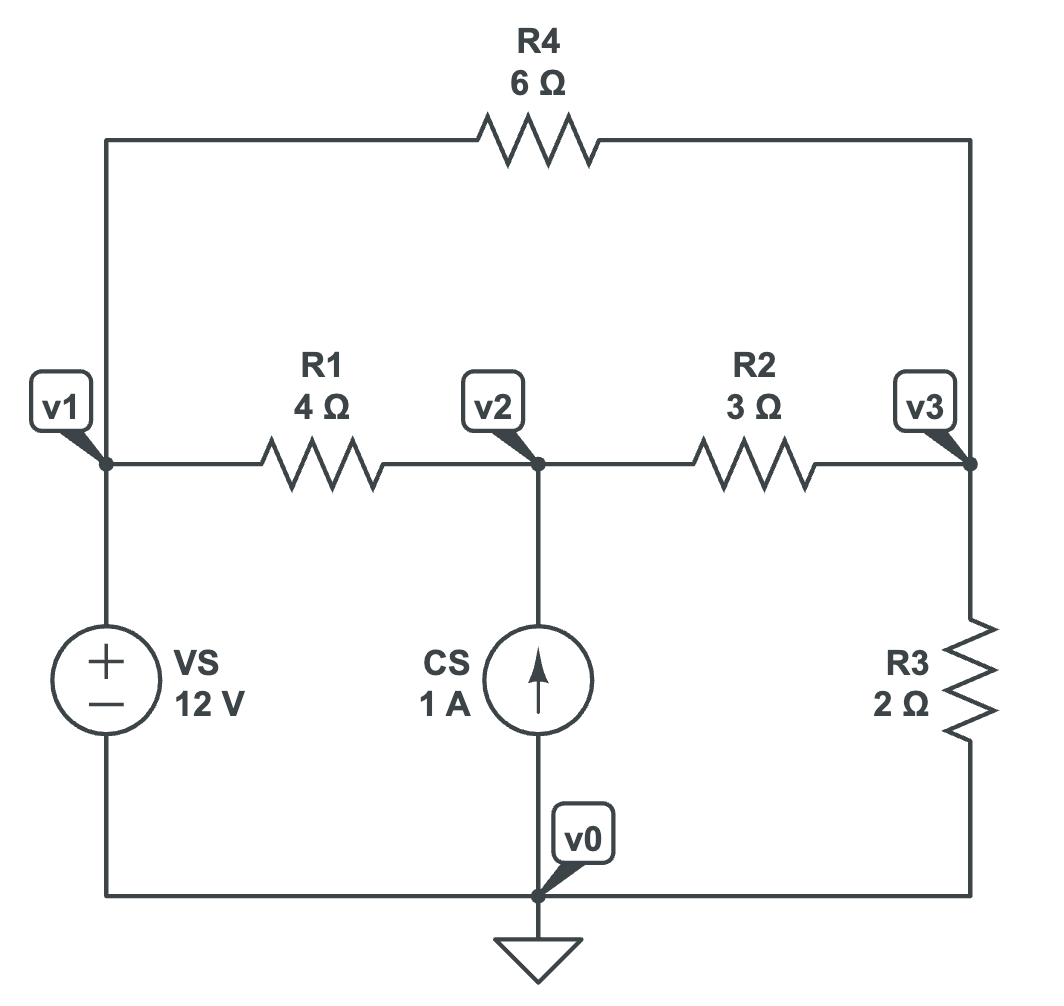
\includegraphics[scale=0.5]{circuit-1.png}
        \caption { Circuit 1}
    \end{center}
\end{figure}

Consider the voltages at the specified nodes in Figure (1). We can apply nodal analysis to determine the voltages at each node and then utilize CircuitLab to simulate the circuit and confirm our results.

Following the path $ v_0 \rightarrow v_s \rightarrow v_1$, we see that $v_1 = 12V$. Applying Kirchhoff's current law (KCL) to $v_2$, we get the node equation

\begin{equation}
    \begin{split}
        \frac{v_2 - 12}{4} + \frac{v_2 - v_3}{3} - 1 = 0 \implies 4v_2 - v_3 = 48
    \end{split}
\end{equation}

Applying KCL to node $v_3$ we get

\begin{equation}
    \begin{split}
        \frac{v_3 - 12}{4} + \frac{v_3 - v_2}{3} + \frac{v_3}{2} = 0 \implies -4v_2 + 13v_3 = 36
    \end{split}
\end{equation}

\end{document}